\textbf{{1.生产者-消费者问题}}

生产者-消费者问题是著名的进程同步问题。它描述的是\textbf{一组生产者向一组消费者提供产品,他们共享一个有界缓冲区,生产者向其中投入产品},消费者从中取走产品。{生产者-消费者问题的同步程序结构描述如下:}

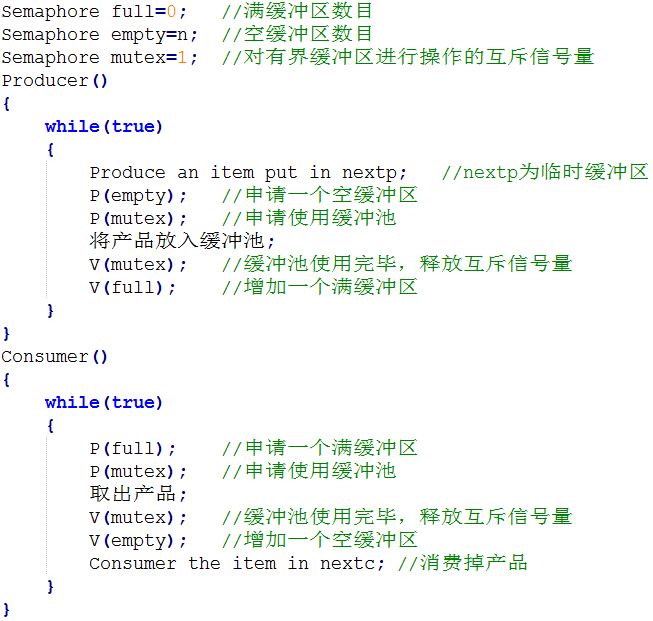
\includegraphics[width=3.33333in,height=3.16667in]{png-jpeg-pics/2D9EBB3BBC8877B96131881E8416729B.png}\\
\textbf{{2.读者-写者问题}}\\
有一个许多进程共享的数据区,这个数据区可以是一个文件或者主存的一块空间;有一些只读取这个数据区的进程(读者)和一些只往数据区写数据的进程(写者),此外还需要满足以下条件:\\
a. 任意多个读者可以同时读这个文件。\\
b. 一次只能有一个写者可以往文件中写(写者必须互斥)。\\
c.
如果一个写者正在进行操作,禁止任何读进程读文件和其他任何写进程写文件。\\
需要分多种情况实现该问题:读者优先、公平情况和写者优先。这里只给出读者优先算法,其他两种情况请参考《操作系统高分笔记》;读者-写者问题的读者优先算法{的同步程序结构描述如下:}\\
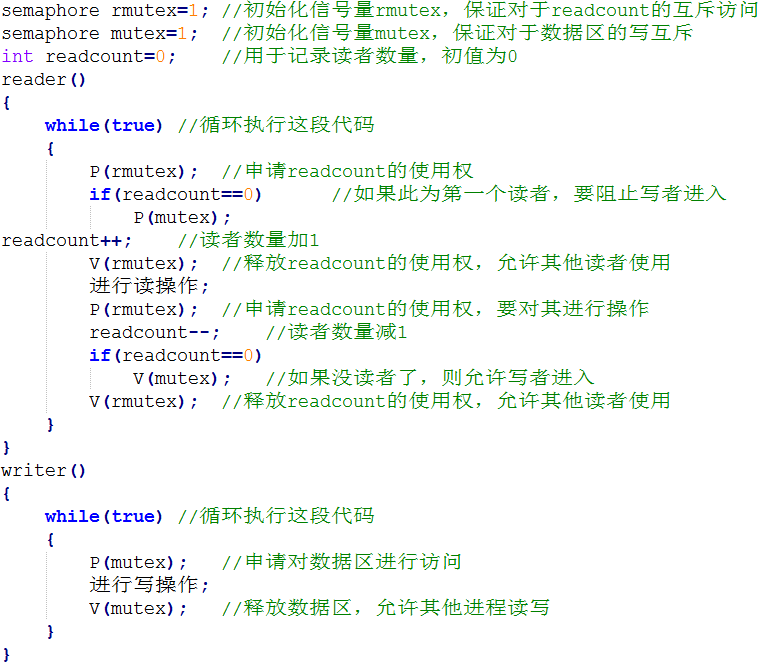
\includegraphics[width=3.33333in,height=2.91667in]{png-jpeg-pics/C9D8567B9541037A8AE5C32D263DFE78.png}\\
\textbf{{3.哲学家进餐问题}}\\

5个哲学家围绕一张圆桌而坐,桌子上放着5根筷子,每两个哲学家之间放一根;哲学家的动作包括思考和进餐,进餐时需要同时拿起他左边和右边的两根筷子,思考时则同时将两根筷子放回原处。哲学家进餐问题可以看做是并发进程执行时处理临界资源的一个典型问题。哲学加进餐问题的同步程序结构描述如下:

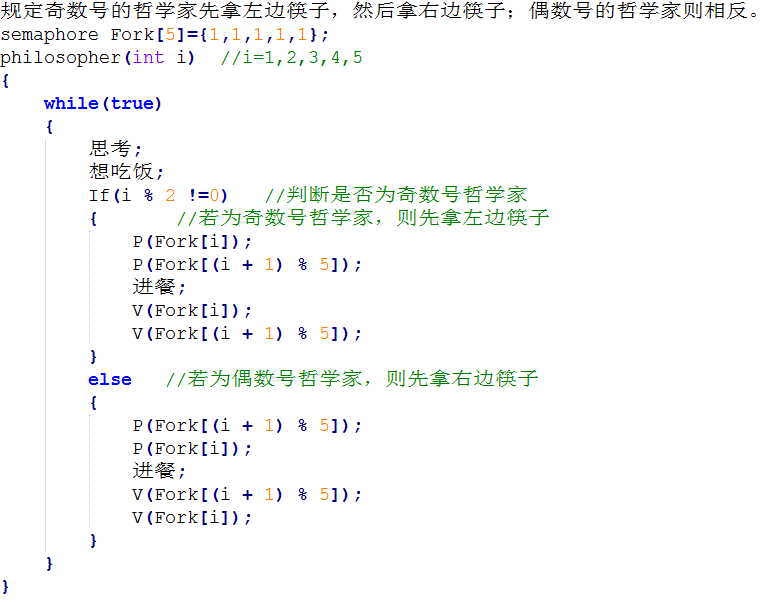
\includegraphics[width=3.33333in,height=2.63542in]{png-jpeg-pics/FB3C7B1684379C75AE7C6A1E15CA2C42.png}\\
\textbf{{4.理发师问题}}\\
理发店有一位理发师、一把理发椅和若干供顾客等候用的凳子(这里假设有n个凳子)。如果没有顾客,则理发师在理发椅上睡觉。当一个顾客到来时,他必须先叫醒理发师;如果理发师正在给顾客理发,则如果有空凳子,该顾客等待;如果没有空凳子,顾客就离开。要为理发师和顾客各设计一段程序来描述其活动。理发师{问题的同步程序结构描述如下:}\\

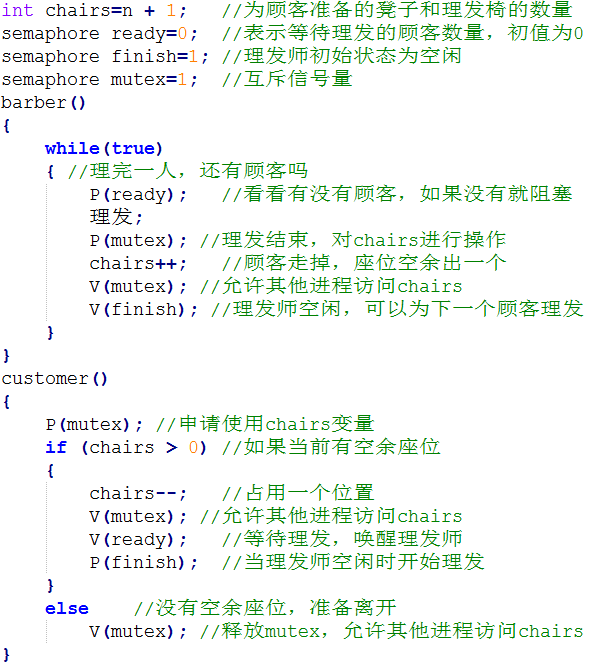
\includegraphics[width=3.33333in,height=3.76042in]{png-jpeg-pics/DF23E2EB33D39390BDB5AD2840A4BD2C.png}\\
